
% @author Jan Robert Rösler 
%
\chapter{Neuronale Navigation mit Bilddaten}

\section{Relevante Technik/Hintergrund}
Hier erfolgt zunächst eine kurze Beschreibung der für Neuronale Navigation auf Bilddaten relevanten Technik. Grundlegendes wird nur der Vollständigkeit halber erwähnt, speziellere Aspekte kurz vorgestellt. 

\subsection{Deep Learning}
Im Bereich des Maschinellen Lernens stellt das Deep Learning einen besonders populären Subbereich dar. Viele bekannte Anwendungen, die in den Medien auch als Künstliche Intelligenz bezeichnet werden, nutzen diese Technik. Eine Hierarchie aus Konzepten zu bauen, bei denen komplizierte Konzepte aus dem Produkt vieler einfacher Konzepte entstehen, erwies sich für das Lernen von Datenrepräsentationen als besonders geeignet. Diese Aufeinanderschichten von Berechnungsschritten in so genannten Layern, bildet ein tiefer Graph ab, auch Neuronales Netz genannt. Die Bezeichnung Deep Learning bezieht sich auf diese Struktur, mit der das Wissen aus Erfahrungswerten, den Trainingsdaten, extrahiert werden kann.\\
Deep Learning gliedert sich selbst in viele Unterthemen auf, eine Darstellung der Geschichte und Technikentwicklung soll hier nicht gegeben werden. Basiswissen zu maschinellem Lernen wird vorausgesetzt, Deep Learning im Speziellen wird in entsprechender Literatur detailliert erklärt, für diese Arbeit diente vor allem ein Hauptbuch (\cite{Goodfellow-et-al-2016}) als begleitende Wissenquelle.


\subsection{CNN}
\textit{Convolutional Neural Networks}, oder kurz CNN, haben sich gerade im Bereich der Bildverarbeitung als überlegen bewiesen. Aus der Biologie inspiriert, findet hier besonders das Prinzip des rezeptiven Feldes Anwendung. Die Aktivität jedes Neurons wird mithilfe einer Faltung berechnet, räumliche Informationen und Zusammenhänge werden so besser erhalten. 2012 konnte ein CNN, AlexNet \cite{krizhevsky2012imagenet}, beim ImageNet-Wettbewerb den Benchmark-Rekord von 25,8 \% auf 16,4 \% drücken, seitdem sind alle gut platzierten Modelle CNNs. Nicht nur in der Bilderkennung, sondern auch in der Spracherkennung (Parsen, Satzmodellierung, Machinelle Übersetzung) gelten CNNs als State-of-the-Art Methode und finden Anwendung in modernsten Technologien.\\
CNNs sollen hier nicht detailliert erklärt werden, das Verständnis wird als Grundlage vorausgesetzt.

\subsection{ResNet}
\textit{Residual Neural Networks}, oder kurz ResNet, ist eine weitere Technik, die ihren Ursprung in der Biologie hat. Das Verhalten so genannter Pyramidenzellen, Nervenzellen im menschlichen Gehirn, wird nachgebildet, indem Abkürzungen zwischen Layer eingebaut werden. Residual Netze wurden 2015 entwickelt, insbesondere ließ sich mit diesem Ansatz das Trainieren tiefer Netze verbessern \cite{DBLP:journals/corr/HeZRS15}. Abbildung~\ref{img:ResBlock} zeigt den schematischen Aufbau eines so genannten Residual Blocks. 

\begin{figure}[h]
	\centering
	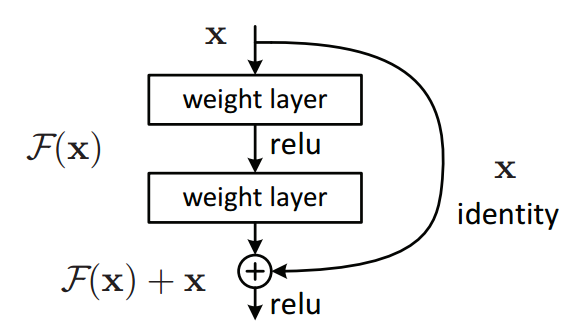
\includegraphics[scale=0.5]{figures/ResidualBlock.png}
	\caption{Residual Block}
	Quelle: \citeI{ResBlock}
	\label{img:ResBlock}
\end{figure}

Je tiefer ein Neuronales Netz ist, desto schwieriger wird das Trainieren aller Layer, ein Problem in diesem Zusammehang ist das \glqq Vanishing Gradient Problem \grqq{}. Für tiefe Layer wird der berechnete Gradient so verschwindend klein, dass irgendwann keine Änderung der Gewichte in den Layern mehr stattfindet, so stagniert das Training und es können keine weiteren Fortschritte erzielt werden.\\
Der Residual-Ansatz fügt einem normalen Block gewichteter Layer eine Abkürzung hinzu. Wie in Abbildung~\ref{img:ResBlock} zu sehen, wird der Input x des Blocks direkt auf den Output addiert. Nimmt man an, dass es für den Input x eine richtige Gewichtsverteilung H(x) der Layer im Block gibt, die erlernt werden soll, dann ist der Unterschied zwischen dem Input und dieser optimalen Verteilung F(x)=H(x)-x. F(x) ist das \glqq Residual \grqq{}, stellt man die Funktion um, erhält man H(x)=F(x)+x. Statt der optimalen Gewichtsverteilung für den Block, lernt das Netz jetzt F(x), also gerade den Unterschied zur Identitätsfunktion des Inputs x.\\
Die Annahme der Autoren (\cite{DBLP:journals/corr/HeZRS15}) war, dass diese Residual-Funktion besser zu erlernen sei, als das originale Mapping. Selbst wenn das gelernte Residual F(x)=0, bekommt man für den Input x immernoch die Identitätsfunktion, also x selbst heraus. Das dieses Mapping meistens näher an der gewünschten optimalen Gewichtsverteilung liegt, war eine weitere Annahme.\\
In Versuchen mit Neuronalen Netzen verschiedener Tiefe konnten diese Annahmen bestätigt werden. 


\subsection{Fine tuning}
Fine Tuning beschreibt einen Prozess, in dem ein bereits trainiertes Neuronales Netz für eine ähnliche Aufgabe abgestimmt wird. Dabei können Teile der Layer des ursprünglichen Netzes ersetzt werden, oder neue hinzugefügt werden. Insbesondere bei Klassifizierungsaufgaben wird dazu häufig die Kategorisierung verändert, um zum Beispiel die von einem Netz erlernten Eigenschaften auf neue Kategorien anzuwenden.\\
In diesem Zusammenhang wird auch \glqq Layer-Freezing \grqq{}, also das einfrieren von Layern vor dem Training verwendet. Eingefrorene Layer aktualisieren ihre Gewichte nicht und sind damit vom Trainingsprozess ausgeschlossen. So soll verhindert werden, dass bereits erlernte Eigenschaften eines Netzes, wie \glqq Katzenohr \grqq{} oder auch \glqq Linie \grqq{} nicht verloren gehen. Dazu werden frühere Layer meist eingefroren, spätere auf einem neuen Datensatz trainiert, um die bereits erlernten Eigenschaften zu nutzen und nicht zu verändern und Eigenschaften für die neue, ähnliche Aufgabe zu erlernen.


\section{Ansätze}
Im folgenden wird auf zwei Ansätze der Navigation mit Neuronalen Netzen eingegangen, durch Gegenüberstellung erster Versuche mit einem modernen Ansatz soll folgenden Ausarbeitungen ein Rahmen gegeben werden.

\subsection{ALVINN}

Versuche durch neuronale Verarbeitung von reinen Bilddaten in einem Szenario zu navigieren, gab es bereits 1989 in Pomerleau's Arbeit, die man auf diesem Gebiet als Pionierarbeit verstehen kann\cite{pomerleau1989alvinn}.
Das Netzwerk \gls{ac:alvinn} sollte das \gls{gl:navlab} steuern, ein Testfahrzeug für Autonome Navigation der Carnegie Mellon University.
In \ref{img:ALVINNa} lässt sich die Architektur nachvollziehen. 
Der rein visuelle Input (die Blautstufenintensität eines Pixels bestimmt das Aktivierungslevel des Inputneurons) wird untersützt durch eine laserbasierte Abstandsmessung und ein Inputneuron für die Kodierung der \glqq Straßenintensität\grqq{}, also ob die Straße heller oder dunkler wird.
Aus heutiger Sicht ist das Netz mit nur einer hidden Layer mit 29 Neronen sehr klein, die im weiteren angesprochenen Architekturen haben deutlich mehr Layer und mehrere Hunderttausend Parameter. 
Zudem interpretiert ALVINN die Aufgabe des Spurfolgens nicht als Regressionsproblem, sondern als Klassifikation. Die Ausgangsneuronen sind eine lineare Repräsentation der Lenkrichtung, die das Fahrzeug in Richtung Fahrbahnmitte steuert. Neuronen in der Mitte stehen für eine Fahrt geradeaus, Neuronen links und rechts für die jeweilige Fahrtrichtung.
Grob gesagt gibt das Neuron mit dem höchsten Aktivierungslevel die Fahrtrichtung (den einzuschlagenden Lenkwinkel) an.
Im Ergebnis konnte das Netz nach 40 Epochen Training auf simulierten Fahrbahnbildern, zu sehen in \ref{img:ALVINNb}, einen 400 Meter Weg durch einen Wald mit \SI{1/2}{\meter/\second} sicher abfahren.


\begin{figure}
	\centering
	\begin{subfigure}{.5\textwidth}
	\centering
		  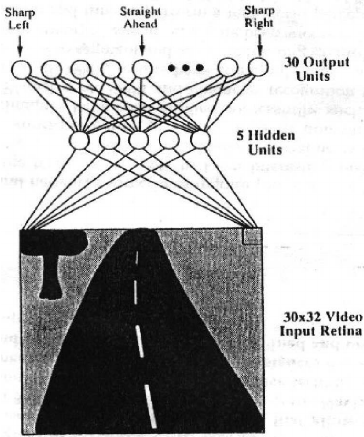
\includegraphics[width=.85\linewidth]{figures/Architecture-ALVINN.png}
		  \caption{}
		  \label{img:ALVINNa}
	\end{subfigure}%
	\begin{subfigure}{.5\textwidth}
	\centering
		  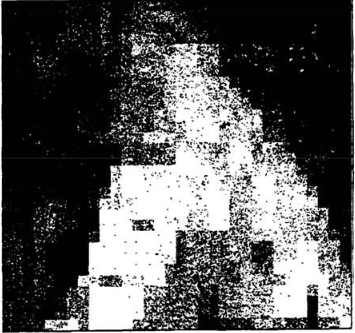
\includegraphics[width=.85\linewidth]{figures/Strasse-ALVINN.png}
	 	  \caption{}
		  \label{img:ALVINNb}
	\end{subfigure}%
	\caption{ALVINN Architektur (a) und simulierte Fahrbahn (b)}
	%Quelle: \protect\citeI{Architecture-ALVINN}
	\label{img:ALVINN}
\end{figure}

\subsection{NVIDIA DAVE-2}

Forschungserkenntnisse der folgenden Jahre trieben die technische Entwicklung voran, auch im Bereich der autonomen Navigation tat sich viel. Zur Orienterung wird eine aktuellere Forschungsarbeit vorgestellt, die einige Aufmerksamkeit auf sich zog.
Im Jahr 2016 veröffentlicht das Technologieunternehmen \textsc{NVIDIA} einen eigenen Ansatz \cite{bojarski2016end}, basierend auf Versuchen mit dem \glqq DARPA Autonomous Vehicle \grqq{} (DAVE) \citeI{DarpaDave} wird dieser \glqq Dave-2 \grqq{} genannt.//
Daten werden hier durch Fahrten auf echten Straßen gesammelt, wofür drei Kameras in der Windschutzscheibe eines Autos angebracht und Steuerungsdaten über den CAN-Bus des Fahrzeuges ausgelesen werden. Mit diesen Daten wird ein CNN trainiert (\ref{img:NVIDIA}), was dann an einer Straßen-Simulation getestet wird. Hervorzuheben ist hier besonders die Verwendung von Convolutional Neural Networks (CNN) und die, im Gegensatz zum bereits erwähnten Ansatz 27 Jahre zuvor, stark gesteigerte Rechenleistung. Folglich können nicht nur Bilder besserer Qualität verarbeitet werden, die Netzarchitektur mit 9 Layern und 250.00 Parametern wäre 1989 nicht in annehmbarer Zeit trainierbar gewesen. Außerdem stellt sich NVIDIA dem Anspruch, eine neuronale Steuerung für öffentliche Straßen zu entwerfen, nicht nur für ein sehr begrenztes Testszenario.\\
Abbildung~\ref{img:NVIDIA} zeigt die Komponenten des Trainingsprozesses. 

\begin{figure}[h]
	\centering
	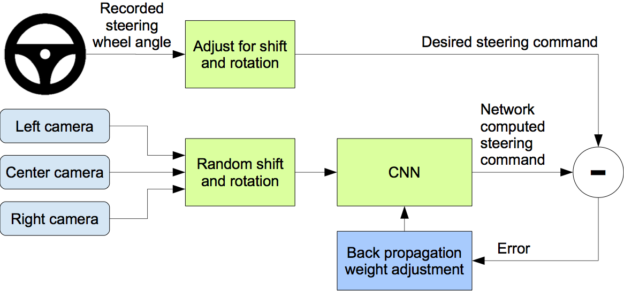
\includegraphics[scale=0.6]{figures/NVIDIA-Training.png}
	\caption{Komponenten des Trainings}
	Quelle: \citeI{NVIDIA-Components}
	\label{img:NVIDIA}
\end{figure}

Mit dem so tranierten CNN wurden sehr gute Ergebnisse erzielt. Sowohl in der Simulation, als auch auf Testfahrten in realen Straßensituationen, steuerte das neuronale Netz ein Auto nahezu fehlerfrei.
Einige der Ansätze und Erkenntnisse aus dieser Arbeit lasse ich für den Entwurf und die Bewertung meiner Arbeit mit einfließen.



